\documentclass{article}


% if you need to pass options to natbib, use, e.g.:
%     \PassOptionsToPackage{numbers, compress}{natbib}
% before loading neurips_2023

% ready for submission
\usepackage[final]{neurips_2023}

% to avoid loading the natbib package, add option nonatbib:
%    \usepackage[nonatbib]{neurips_2023}


\usepackage[utf8]{inputenc} % allow utf-8 input
\usepackage[T1]{fontenc}    % use 8-bit T1 fonts
\usepackage{hyperref}       % hyperlinks
\usepackage{url}            % simple URL typesetting
\usepackage{booktabs}       % professional-quality tables
\usepackage{amsfonts}       % blackboard math symbols
\usepackage{nicefrac}       % compact symbols for 1/2, etc.
\usepackage{microtype}      % microtypography
\usepackage{xcolor}         % colors
\usepackage{graphicx}       % addtional package for show figures


\begin{document}


\maketitle


%%%%%%% Part 4 Text Features Start %%%%%%%%%

\section{Text Features}

\subsubsection{(a) Picking $k$ for text embeddings}
We load 35\,826 sentence‑transformer embeddings (1\,024‑D, unit norm). A PCA that keeps 90\,\% of the variance shrinks them to 100 dimensions. We then run $k$‑Means for $k=5\ldots20$. The silhouette curve in Figure~\ref{fig:text_silhouette} reaches a local maximum at $k=15$ ($s=0.071$), so we choose \textbf{$k=15$}. The t‑SNE plots in Figure~\ref{fig:text_tsne} show cleaner colour islands for $k=15$ than for $k=11$.

\begin{figure}[h]
  \centering
  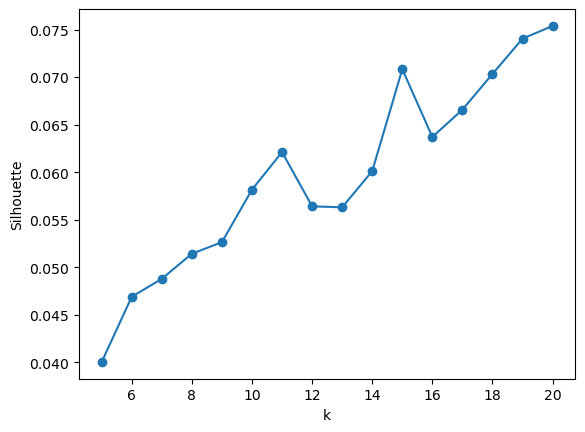
\includegraphics[width=.55\linewidth]{figs_tang/04_silhouette_k.png}
  \caption{Silhouette over $k=5\ldots20$ (text embeddings).}
  \label{fig:text_silhouette}
\end{figure}

\begin{figure}[h]
  \centering
  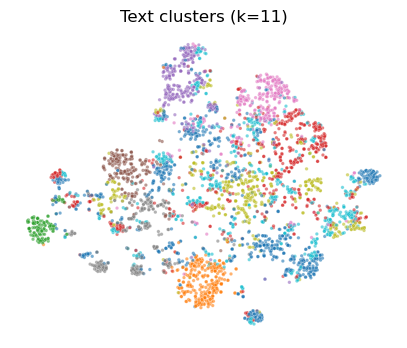
\includegraphics[width=.45\linewidth]{figs_tang/04_text_cluster11.png}\hfill
  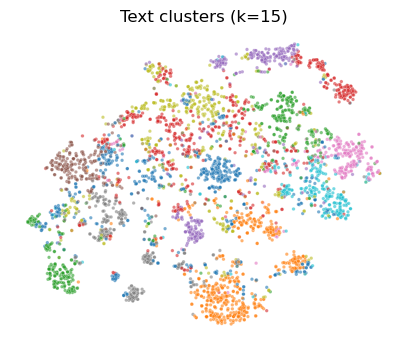
\includegraphics[width=.45\linewidth]{figs_tang/04_text_cluster15.png}
  \caption{t‑SNE colour map of text clusters for $k=11$ (left) and $k=15$ (right).}
  \label{fig:text_tsne}
\end{figure}

\subsubsection{(b) Themes of the 15 clusters}
We listen to five random clips in every cluster. Table~\ref{tab:text_themes} lists the main sound we hear: bells (\texttt{C0}), sirens or buzzing (\texttt{C1}), dogs or birds (\texttt{C2}), water or rain (\texttt{C3}), etc. This quick check tells us the clusters are semantically meaningful.

\begin{table}[h]
  \caption{Manual auditory label of the 15 text clusters.}
  \label{tab:text_themes}
  \centering
  \small
  \begin{tabular}{cl}
    \toprule
    Cluster & Dominant sound theme \\ \midrule
    0 & bell sound \\
    1 & buzzing sound / siren \\
    2 & dogs or birds \\
    3 & water / rain \\
    4 & repeating mechanical sound \\
    5 & vocal sound \\
    6 & engine / vehicle \\
    7 & high‑pitched vocal (kitten / child) \\
    8 & high‑pitched noise / drill \\
    9 & high‑level ambience \\
    10 & hissing / scratching \\
    11 & generic animal farm / birds \\
    12 & high‑pitched repeating motor \\
    13 & rhythmic footsteps / cheering \\
    14 & low‑level ambience / jazz \\
    \bottomrule
  \end{tabular}
\end{table}

\subsubsection{(c) Dog \& cat tagging rule}
A simple rule—regex \texttt{(bark$|$woof$|$puppy)} or \texttt{(meow$|$purr$|$kitten)} plus cosine similarity $>0.35$ to class prototypes—finds \textbf{1\,483 dog} and \textbf{731 cat} tags. The entropy for both is 0.073, meaning over 80\,\% of each class sits in only two clusters. Figure~\ref{fig:dogcat_tsne} shows how tightly these points group in t‑SNE space.

\begin{figure}[h]
  \centering
  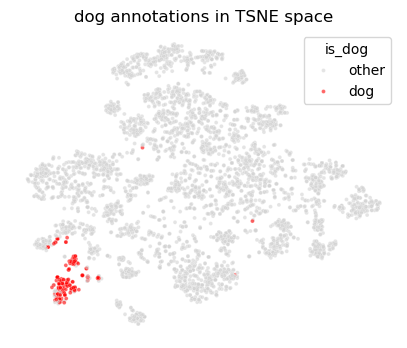
\includegraphics[width=.42\linewidth]{figs_tang/04_dog_annotations_in_tsne_space.png}\hfill
  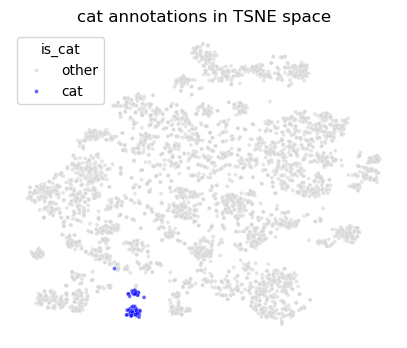
\includegraphics[width=.42\linewidth]{figs_tang/04_cat_annotations_in_tsne_space.png}
  \caption{Dog (left) and cat (right) annotations highlighted in t‑SNE space.}
  \label{fig:dogcat_tsne}
\end{figure}

\subsubsection{(d) Linking text and audio clusters}
The 51\,966 audio region vectors were clustered into four groups (see Section~3c). After matching by \texttt{(filename, onset, offset)} rounded to 1 ms we get 35\,552 event pairs. Four very small text clusters ($<0.3$\,\% each) have no audio match, so their rows are zero in Figure~\ref{fig:text_audio_heat}. The heatmap shows clear links—bells map to audio 0, speech to 1, animal calls to 2, water/ambience to 3. The Normalised Mutual Information is \textbf{NMI = 0.28}.

\begin{figure}[h]
  \centering
  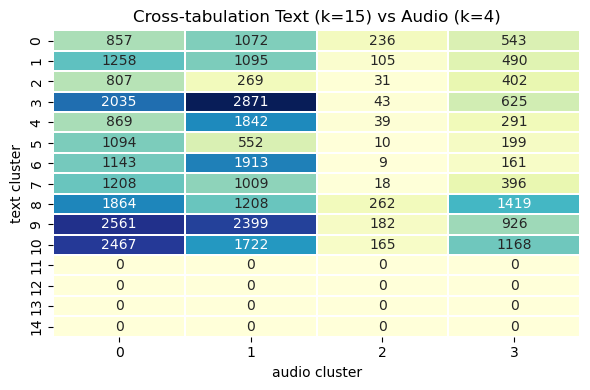
\includegraphics[width=.7\linewidth]{figs_tang/04_text_audio_heatmap_k15.png}
  \caption{Cross‑tabulation of text clusters ($k=15$) vs. audio clusters ($k=4$). Rows 11–14 are empty because those text clusters contain only sub‑frame annotations without audio features.}
  \label{fig:text_audio_heat}
\end{figure}

\paragraph{Take‑aways.} Text embeddings form 15 clear semantic clusters. The dog/cat rule confirms tight grouping. An NMI of 0.28 suggests a moderate but useful link between text and audio spaces, enough to transfer weak labels between them.

%%%%%%% Part 4 Text Features Finish %%%%%%%%%

\end{document}